\title{\bf Lecture 2 - Cryptographic Hash Functions\\}
\author{\bf Rylan Schaeffer and Vincent Yang\\}
\date{\bf \today \\}

\documentclass{article}
\renewcommand{\thesubsection}{\thesection.\alph{subsection}}
\usepackage{enumerate}
\PassOptionsToPackage{hyphens}{url}\usepackage{hyperref}
\usepackage{amsmath}
\usepackage{amssymb}
\usepackage{hyperref}
\usepackage{graphicx}
\setlength{\oddsidemargin}{0in}
\setlength{\evensidemargin}{0in}
\setlength{\textheight}{9in}
\setlength{\textwidth}{6.5in}
\setlength{\topmargin}{-0.5in}

\begin{document}
\maketitle

Note: This lecture is based on Princeton University's BTC-Tech: Bitcoin and Cryptocurrency Technologies Spring 2015 course.

\section*{Terms}
\begin{itemize}
\item Set : group of objects represented as a unit. enumerate, or give way to determine membership in set
\subitem Empty set = set with 0 members
\subitem Cartesian Product or Cross Product (x): tuples of all possible pairs
\item Alphabet : finite, non-empty set
\item String : finite sequence of characters from common alphabet
\subitem empty string $\varepsilon$ (string of length zero)
\subitem concatenation by joining or $|$, can use exponent for repeat concatenation
\item Language : set of strings over common alphabet
\item Kleene star (Kleene operator, Kleene closure) : either on sets of strings or sets of characters. Means "zero or more". More formally:
\subitem $V_0 = \{\varepsilon\}$
\subitem $V_1 = V$
\subitem $V_{i+1} = \{ wv : w \in V_i and v \in V \}$ for i $>$ 0
\subitem $V^* = \bigcup\limits_{i \in \mathbb{N}} V_i$
=======
  \item Set : group of objects represented as a unit
  \item Alphabet : finite, non-empty set
  \item String : finite sequence of characters from common alphabet, including empty string $\varepsilon$
  \item Language : set of strings over common alphabet
\end{itemize}

\section*{Hash Functions}
\begin{itemize}
  \item $H: \{0,1\}^* \rightarrow \{0,1\}^k$, for fixed k e.g. 256
  \item Should be efficiently computable O(n)
  \item Examples: mod operator, separate chaining hash (draw)
  \item Homework 1 - \emph{SHA-256}
\end{itemize}

\section*{Cryptographic Hash Function}
Two additional properties
\begin{itemize}
  \item Collision Resistant: Computationally infeasible to find $x, y$ such that $x \neq y$ and $H(x) = H(y)$
    \subitem mod operator is not collision resistant
    \subitem collisions exist by pigeonhole principle - hence, computationally infeasible
    \subitem Avalanche Effect - when one letter changes, everything changes
    \subitem can also call "binding," since once hash is published, you cannot replace input value with another input value without modifying the hash output
  \item Hiding: Computationally infeasible to find $x$ given $H_{given}$ such that $H(x) = H_{given}$
    \subitem Frequently, cryptographic hash functions will be called one-way hash functions (trap door functions)
    \subitem Frequently, message space is too small. Append nonce (i.e. random value) r to grow message space such that computationally infeasible to find $x$ such that $H(x|r) = H_{given}$
  \item Birthday paradox reduces difficulty of finding collisions 
    \begin{itemize}
      \item How many people do you need in a room for there to be a 50\% chance that two have the same birthday? (A: 23)
      \item Exponents aren't intuitive
      \item With 23 people we have 253 pairs - $\frac{23 \cdot 22}{2}=253$.
      \item Chance of 2 people having diff. birthdays is $1 - \frac{1}{365} = \frac{364}{365} = .997260$.
      \item If all pairs are different, this is like having 253 heads in a row. $Probability = (\frac{364}{365})\textsuperscript{253} = .4995$.
      \item SHA-256: Let's say we have a "perfect" hash function with output size $n$, with $p$ messages to hash. Probability of collision is $\frac{p\textsuperscript{2}}{2\textsuperscript{n+1}}$.
      \item This means, if we have $n=256$ as in SHA-256, and 1 billion messages ($p = 10\textsuperscript{9})$ then the probability is still only $4.3 \cdot 10\textsuperscript{-60}$.
      \item A mass murdering space rock happens about once every 30 million years. The probability of it happening in the next second is about $10\textsuperscript{-15}$. This is 45 times more likely than a SHA-256 collision.
    \end{itemize}

\end{itemize}

\section*{Applications}
\begin{itemize}
  \item Message Digest
    \subitem Create summary (or ``digest") of block of text
    \subitem Suppose I have $msg$ and $H$ is a cryptographic hash function. Then I know that $H(msg)$ or perhaps $H(msg|r)$ (where r is a random value and is needed because the message is predictable), will produce a hash value that no other block of text will.
    \subitem Example: cryptographic checksums
  \item Commitments
    \subitem Analogous to sealed envelope on the table
    \subitem Hiding ensures no one can "reverse engineer" the contents. Collision-resistant guarantees to the other party that you are bound to the value you initially put in.
\end{itemize}

\section*{Puzzle Friendliness}
\begin{itemize}
  \item Search Puzzle
    \subitem Given $H$, target set $Y$, and value $x$
    \subitem Goal: find r such that $H(x|r) \in Y$
  \item Puzzle friendly if no solving strategy for puzzle other than trying random guesses at $r$
  \item Examples: $0|\{0,1\}^{k-1}$, $00|\{0,1\}^{k-1}$, $000|\{0,1\}^{k-1}$
    \subitem P(l leading zeroes) = $\frac{1}{2^l}$, can use geometric distribution's cumulative distribution function to model likelihood of observing a ``hit" after a given number of failures
  \item Useful for mining, which we will get to later
\end{itemize}

\section*{Hash Structures}
\begin{itemize}
  \item Hash pointer : hash of data. Gives way to verify information hasn't changed, much like pointer gives a way to retrieve location of information
  \item Hash linked list (block chain) : Each block has hash of previous block plus new data. Head is hash of most recent block.
    \subitem Tamper-evident log
  \item Hash tree (Merkle Tree) : binary tree of data blocks. Proof of membership and proof of non-membership in $log(n)$, so faster than hash linked list. Can also sort.
    \subitem Verification in $O(log(n))$.
  \item Can combine. Block chain is usually hash linked list of hash trees  (draw picture on board)\\
    \begin{center}
      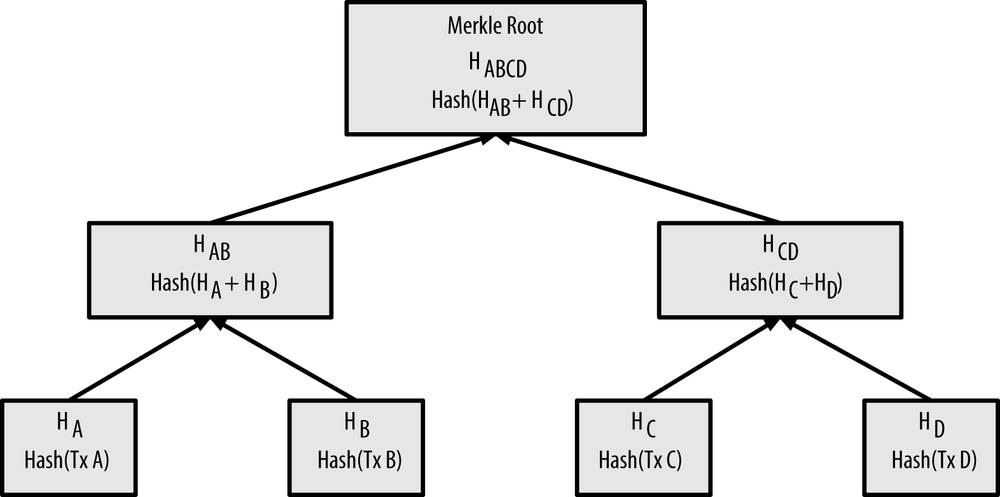
\includegraphics[width=7cm, height=4cm]{merkle.png}
      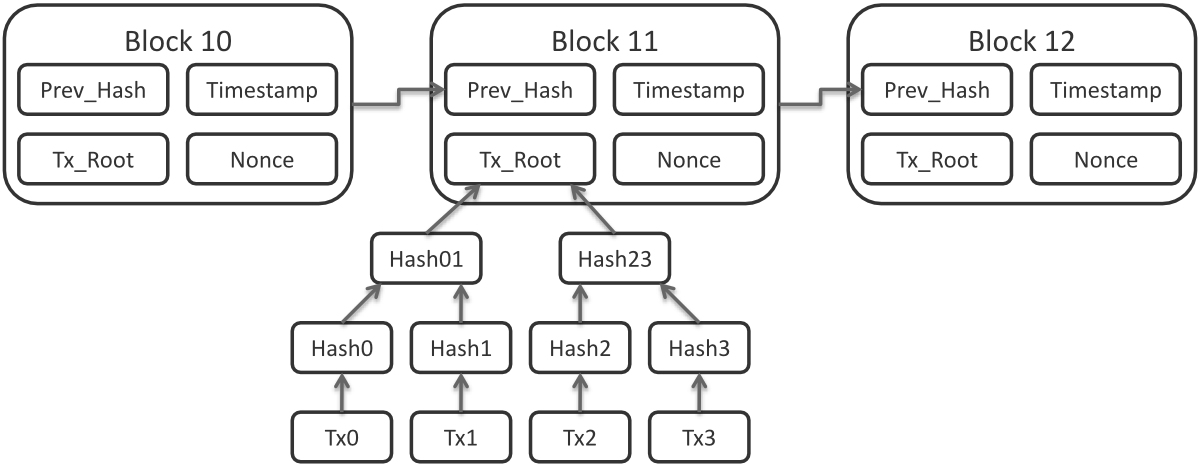
\includegraphics[width=7cm, height=4cm]{block_chain.png}
    \end{center}
\end{itemize}

\section{Actual Cryptographic Hash Functions}
\begin{itemize}
\item Turns out, creating ideal cryptographic hash function is difficult
\item Ron Rivest invented MD4 and MD5 in 1990 and 1991, collisions found
\item SHA-1 designed by NSA in 1993, replaced in 1995. 2005 cryptanalysts found collisions, by 2010 organizations refuse to accept e.g. Google, Microsoft
\item SHA-2 designed by NSA. 2001. Family of functions with different possible digest lengths including 224, 256, 384, 512.
\subitem SHA-256 uses Merkle-Damgard transform to turn fixed-length collision-resistant compression function into hash function that accepts arbitrary length inputs (same Merkle as Merkle trees!)
\item SHA-3, released 2015.
\end{itemize}

\section*{SHA-256}
\begin{itemize}
  \item Merkle-Damgard Transform: change arbitrary length to fixed length - compression function
  \item Takes input length $m$ and output length $n$.
    \begin{enumerate}
      \item Split input into blocks of length $m-n$.
      \item Pass each block in with output of previous block
      \item Use IV (initialization vector) for first block
      \item Return last block's output
      \item Padding: 
        \begin{enumerate}
          \item Append $1$ to the end
          \item Append $k$ bits of $0$ such that $k$ is the smallest integer that fulfills $(l + 1 + k)\ mod\ 512\ =\ 448$; $l$ is length of message.
          \item Add length $l < 2\textsuperscript{64}$ represented with 64 bits, added to the end.
          \item Message is \emph{always} padded.
        \end{enumerate}
    \end{enumerate}
  \item Feistel Network/Cipher (2 rounds; SHA is 8)
    \begin{enumerate}
      \item F is the round function, and K0, K1, ... Kn are the keys for rounds 0, 1, ... n. 
      \item Split plaintext to 2 blocks L0 and R0
      \item For reach round i = 0, 1, ..., n, compute:
        \subitem $L_{i+1}\ =\ R_{i}$
        \subitem $R_{i+1}\ =\ R_{i+1} \oplus F(R_{i}, K_{i})$.
      \item Ciphertext is $(R_{n+1}, L_{n+1})$
    \end{enumerate}
  \item After padding from above, split into smaller parts, XOR with each other, left bitshift.
    \begin{center}
      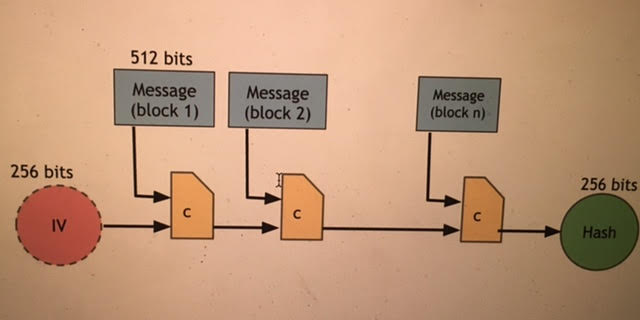
\includegraphics[width=8cm, height=3cm]{sha.jpg}
    \end{center}
    Other Sources: (More SHA) \url{http://www.quadibloc.com/crypto/mi060501.htm}
\end{itemize}
\end{document}
